\section{Customizing the GUI}
\label{Qtmodules}
\index{modules, custom GUI}

The code that creates the GUI for a \texttt{DefaultGUIModel}-derived user module is located within the \texttt{createGUI()} member function. This function can be overloaded by a derived class to generate a custom GUI. RTXI uses the Qt platform, which is open-source and has a very well-documented API for creating GUI controls). Qt also uses a signal-and-slots architecture in which interactions with these GUI elements, such as pushing a button, emits a signal that can then be connected to a function. Whenever an event occurs, the slot function is executed. This architecture is made possible by a C++ preprocessor called MOC that generates additional *.cpp implementation and *.h header files for each class that has these features. These additional source files must also be listed in the Makefile.

There are several options available to users seeking to build their own GUIs. The simplest by far is to leave everything to \texttt{DefaultGUI}'s \texttt{createGUI} function. Customization options are also available through the \texttt{customizeGUI} function and overriding the \texttt{createGUI} function altogether. The following describes GUI creation in the context of the Neuron module. 

\attention The latter option is generally not recommended. If possible, rely on \texttt{customizeGUI}. 

\subsection{Leave everything to \texttt{createGUI}}
The Neuron module's GUI is automatically generated by DefaultGUIModels's \texttt{createGUI} function. It operates by taking each \texttt{PARAMETER},  \texttt{STATE}, \texttt{EVENT}, and \texttt{COMMENT} variable in \texttt{vars[]} and creating a row in the GUI containing the variable name and stored value. After that, the utility buttons ("Pause", "Modify", and "Unload") are added to the bottom. \texttt{createGUI} should be adequate for simple modules, such as Neuron. In other words, no GUI configuration is necessary. For more complex modules, use \texttt{customizeGUI}. 

\subsection{Use \texttt{customizeGUI}}

To understand how to use \texttt{customizeGUI}, it is important to understand the format of the GUI. For all of its windows, RTXI uses Qt. When RTXI is opened, one large window is displayed, and every module is opened as a subwindow within it. Each subwindow has its own formatting styles, set in source code. \texttt{DefaultGUIModel} uses \texttt{QGridLayout} to define elements within its subwindow. \texttt{QGridLayout} splits windows into cells indexed by row and column. Users can then place items in any cell or combination of contiguous cells. The \texttt{createGUI} function generates the column of variables with values and then the utility buttons and places them respectively in cells (1,0) and (2,0). The \texttt{customizeGUI} function takes the window created by \texttt{customizeGUI} and allows users to place additional elements in any positions that are not (1,0) and (2,0). Below is one example of a possible grid configuration.

\begin{figure}[h!] 
\begin{center}
\label{QGridLayout}
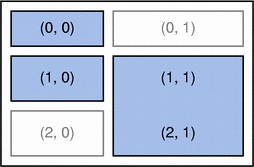
\includegraphics[width=3in]{examplegrid.png} 
\caption[Example QGridLayout]{\texttt{QGridLayout} allows users to add elements to a window in a grid structure. The top-left corner is (0,0), and users can insert widgets spanning however many rows and columns in however many rows and columns.} 
\end{center}
\end{figure}

As is, Neuron does not use \texttt{customizeGUI}. Suppose, though, that we wanted to add two buttons in a row above the parameters. The syntax would be as follows:

\begin{maxipage}
\begin{example}
\hspace{0cm}void Neuron::customizeLayout(void) \{\\
\hspace{.5cm}QGridLayout *customlayout = DefaultGUIModel::getLayout();\\
\hspace{.5cm}\\
\hspace{.5cm}QGroupBox *buttongroup = new QGroupBox;\\
\hspace{.5cm}QHBoxLayout *buttonlayout = new QButtonLayout;\\
\hspace{.5cm}QPushButton *aBttn = new QPushButton("Button A", buttonlayout);\\
\hspace{.5cm}QPushButton *bBttn = new QPushButton("Button B", buttonlayout);\\
\hspace{.5cm}buttongroup->setLayout(buttonlayout);\\
\hspace{.5cm}\\
\hspace{.5cm}customlayout->addWidget(buttongroup, 0, 0)\\
\hspace{.5cm}setLayout(customlayout);\\
\}\\
\end{example}
\end{maxipage}

The first and last two commands are necessary for \texttt{customizeLayout} to function. The first one grabs the window object created by \texttt{createGUI} and assigns it to \texttt{customlayout}. The middle section defines the elements to be added to the GUI. These are all Qt-defined classes for which documentation is freely available online (http://qt-project.org/doc/qt-4.8/). The second-to-last line assigns the GUI elements to the window. It specifies position (0,0), so the buttons will be displayed in the top left corner. The last line sets the GUI to the newly modified one. 